\documentclass[twoside]{book}

% Packages required by doxygen
\usepackage{fixltx2e}
\usepackage{calc}
\usepackage{doxygen}
\usepackage[export]{adjustbox} % also loads graphicx
\usepackage{graphicx}
\usepackage[utf8]{inputenc}
\usepackage{makeidx}
\usepackage{multicol}
\usepackage{multirow}
\PassOptionsToPackage{warn}{textcomp}
\usepackage{textcomp}
\usepackage[nointegrals]{wasysym}
\usepackage[table]{xcolor}

% Font selection
\usepackage[T1]{fontenc}
\usepackage[scaled=.90]{helvet}
\usepackage{courier}
\usepackage{amssymb}
\usepackage{sectsty}
\renewcommand{\familydefault}{\sfdefault}
\allsectionsfont{%
  \fontseries{bc}\selectfont%
  \color{darkgray}%
}
\renewcommand{\DoxyLabelFont}{%
  \fontseries{bc}\selectfont%
  \color{darkgray}%
}
\newcommand{\+}{\discretionary{\mbox{\scriptsize$\hookleftarrow$}}{}{}}

% Page & text layout
\usepackage{geometry}
\geometry{%
  a4paper,%
  top=2.5cm,%
  bottom=2.5cm,%
  left=2.5cm,%
  right=2.5cm%
}
\tolerance=750
\hfuzz=15pt
\hbadness=750
\setlength{\emergencystretch}{15pt}
\setlength{\parindent}{0cm}
\setlength{\parskip}{3ex plus 2ex minus 2ex}
\makeatletter
\renewcommand{\paragraph}{%
  \@startsection{paragraph}{4}{0ex}{-1.0ex}{1.0ex}{%
    \normalfont\normalsize\bfseries\SS@parafont%
  }%
}
\renewcommand{\subparagraph}{%
  \@startsection{subparagraph}{5}{0ex}{-1.0ex}{1.0ex}{%
    \normalfont\normalsize\bfseries\SS@subparafont%
  }%
}
\makeatother

% Headers & footers
\usepackage{fancyhdr}
\pagestyle{fancyplain}
\fancyhead[LE]{\fancyplain{}{\bfseries\thepage}}
\fancyhead[CE]{\fancyplain{}{}}
\fancyhead[RE]{\fancyplain{}{\bfseries\leftmark}}
\fancyhead[LO]{\fancyplain{}{\bfseries\rightmark}}
\fancyhead[CO]{\fancyplain{}{}}
\fancyhead[RO]{\fancyplain{}{\bfseries\thepage}}
\fancyfoot[LE]{\fancyplain{}{}}
\fancyfoot[CE]{\fancyplain{}{}}
\fancyfoot[RE]{\fancyplain{}{\bfseries\scriptsize Generated by Doxygen }}
\fancyfoot[LO]{\fancyplain{}{\bfseries\scriptsize Generated by Doxygen }}
\fancyfoot[CO]{\fancyplain{}{}}
\fancyfoot[RO]{\fancyplain{}{}}
\renewcommand{\footrulewidth}{0.4pt}
\renewcommand{\chaptermark}[1]{%
  \markboth{#1}{}%
}
\renewcommand{\sectionmark}[1]{%
  \markright{\thesection\ #1}%
}

% Indices & bibliography
\usepackage{natbib}
\usepackage[titles]{tocloft}
\setcounter{tocdepth}{3}
\setcounter{secnumdepth}{5}
\makeindex

% Custom commands
\newcommand{\clearemptydoublepage}{%
  \newpage{\pagestyle{empty}\cleardoublepage}%
}

\usepackage{caption}
\captionsetup{labelsep=space,justification=centering,font={bf},singlelinecheck=off,skip=4pt,position=top}

%===== C O N T E N T S =====

\begin{document}

% Titlepage & ToC
\pagenumbering{roman}
\begin{titlepage}
\vspace*{7cm}
\begin{center}%
{\Large My Project \\[1ex]\large 1.\+0.\+0 }\\
\vspace*{1cm}
{\large Generated by Doxygen 1.8.11}\\
\end{center}
\end{titlepage}
\clearemptydoublepage
\tableofcontents
\clearemptydoublepage
\pagenumbering{arabic}

%--- Begin generated contents ---
\chapter{Data Structure Index}
\section{Data Structures}
Here are the data structures with brief descriptions\+:\begin{DoxyCompactList}
\item\contentsline{section}{\hyperlink{structlist}{list} }{\pageref{structlist}}{}
\item\contentsline{section}{\hyperlink{structthing}{thing} }{\pageref{structthing}}{}
\end{DoxyCompactList}

\chapter{File Index}
\section{File List}
Here is a list of all files with brief descriptions\+:\begin{DoxyCompactList}
\item\contentsline{section}{/home/zerfalex/22/so/trab/include/{\bf data\+Structs.\+h} \\*Header file with data structure A\+PI }{\pageref{data_structs_8h}}{}
\item\contentsline{section}{/home/zerfalex/22/so/trab/include/{\bf processor.\+h} }{\pageref{processor_8h}}{}
\item\contentsline{section}{/home/zerfalex/22/so/trab/include/{\bf transform.\+h} \\*Header file with functions to transform notebook data into data\+Structs data }{\pageref{transform_8h}}{}
\item\contentsline{section}{/home/zerfalex/22/so/trab/src/{\bf main.\+c} }{\pageref{main_8c}}{}
\item\contentsline{section}{/home/zerfalex/22/so/trab/src/lib/{\bf data\+Structs.\+c} }{\pageref{data_structs_8c}}{}
\item\contentsline{section}{/home/zerfalex/22/so/trab/src/lib/{\bf processor.\+c} }{\pageref{processor_8c}}{}
\item\contentsline{section}{/home/zerfalex/22/so/trab/src/lib/{\bf transform.\+c} }{\pageref{transform_8c}}{}
\end{DoxyCompactList}

\chapter{Data Structure Documentation}
\hypertarget{structlist}{}\section{list Struct Reference}
\label{structlist}\index{list@{list}}
\subsection*{Data Fields}
\begin{DoxyCompactItemize}
\item 
int \hyperlink{structlist_a439227feff9d7f55384e8780cfc2eb82}{size}
\item 
G\+Ptr\+Array $\ast$ \hyperlink{structlist_a3167491f9e7a19c8575b456fb7830733}{array}
\end{DoxyCompactItemize}


\subsection{Detailed Description}


Definition at line 10 of file data\+Structs.\+c.



\subsection{Field Documentation}
\index{list@{list}!array@{array}}
\index{array@{array}!list@{list}}
\subsubsection[{\texorpdfstring{array}{array}}]{\setlength{\rightskip}{0pt plus 5cm}G\+Ptr\+Array$\ast$ array}\hypertarget{structlist_a3167491f9e7a19c8575b456fb7830733}{}\label{structlist_a3167491f9e7a19c8575b456fb7830733}


Definition at line 12 of file data\+Structs.\+c.

\index{list@{list}!size@{size}}
\index{size@{size}!list@{list}}
\subsubsection[{\texorpdfstring{size}{size}}]{\setlength{\rightskip}{0pt plus 5cm}int size}\hypertarget{structlist_a439227feff9d7f55384e8780cfc2eb82}{}\label{structlist_a439227feff9d7f55384e8780cfc2eb82}


Definition at line 11 of file data\+Structs.\+c.



The documentation for this struct was generated from the following file\+:\begin{DoxyCompactItemize}
\item 
/home/zerfalex/22/so/trab/src/lib/\hyperlink{data_structs_8c}{data\+Structs.\+c}\end{DoxyCompactItemize}

\hypertarget{structthing}{}\section{thing Struct Reference}
\label{structthing}\index{thing@{thing}}


A struct which houses a command\textquotesingle{}s parameters, it\textquotesingle{}s, if parsed, output, reference and sline value.  


\subsection*{Data Fields}
\begin{DoxyCompactItemize}
\item 
int \hyperlink{structthing_a8260a04cd33e11250d7680ccd06af2fc}{sline}
\begin{DoxyCompactList}\small\item\em An int which indicates if the present member is part of a sequence (Same\+L\+I\+NE) \end{DoxyCompactList}\item 
int \hyperlink{structthing_adb528a1cb1ca190150183394d082590d}{ref}
\begin{DoxyCompactList}\small\item\em Indicates which thing\textquotesingle{}s output this one should use as input.  ~\newline
 Is relative to the current position. \end{DoxyCompactList}\item 
char $\ast$ \hyperlink{structthing_a0d119d211b6770402e90c832e7d03767}{params}
\begin{DoxyCompactList}\small\item\em The command\textquotesingle{}s parameters.  ~\newline
 Saves the entirety of the received command, with the exception of sequences which are treated as normal commands which use the previous\textquotesingle{} output. \end{DoxyCompactList}\item 
char $\ast$ \hyperlink{structthing_a47866494eb84961e021291efbea9b569}{output}
\begin{DoxyCompactList}\small\item\em The output after being processed by list\+\_\+process\char`\"{}(\char`\"{}L\+I\+ST list\char`\"{})\char`\"{}. \end{DoxyCompactList}\end{DoxyCompactItemize}


\subsection{Detailed Description}
A struct which houses a command\textquotesingle{}s parameters, it\textquotesingle{}s, if parsed, output, reference and sline value. 

Defines a list of pointers, in this case, a list of T\+H\+I\+N\+Gs. 

Definition at line 24 of file data\+Structs.\+c.



\subsection{Field Documentation}
\index{thing@{thing}!output@{output}}
\index{output@{output}!thing@{thing}}
\subsubsection[{\texorpdfstring{output}{output}}]{\setlength{\rightskip}{0pt plus 5cm}char$\ast$ output}\hypertarget{structthing_a47866494eb84961e021291efbea9b569}{}\label{structthing_a47866494eb84961e021291efbea9b569}


The output after being processed by list\+\_\+process\char`\"{}(\char`\"{}L\+I\+ST list\char`\"{})\char`\"{}. 



Definition at line 28 of file data\+Structs.\+c.

\index{thing@{thing}!params@{params}}
\index{params@{params}!thing@{thing}}
\subsubsection[{\texorpdfstring{params}{params}}]{\setlength{\rightskip}{0pt plus 5cm}char$\ast$ params}\hypertarget{structthing_a0d119d211b6770402e90c832e7d03767}{}\label{structthing_a0d119d211b6770402e90c832e7d03767}


The command\textquotesingle{}s parameters.  ~\newline
 Saves the entirety of the received command, with the exception of sequences which are treated as normal commands which use the previous\textquotesingle{} output. 



Definition at line 27 of file data\+Structs.\+c.

\index{thing@{thing}!ref@{ref}}
\index{ref@{ref}!thing@{thing}}
\subsubsection[{\texorpdfstring{ref}{ref}}]{\setlength{\rightskip}{0pt plus 5cm}int ref}\hypertarget{structthing_adb528a1cb1ca190150183394d082590d}{}\label{structthing_adb528a1cb1ca190150183394d082590d}


Indicates which thing\textquotesingle{}s output this one should use as input.  ~\newline
 Is relative to the current position. 



Definition at line 26 of file data\+Structs.\+c.

\index{thing@{thing}!sline@{sline}}
\index{sline@{sline}!thing@{thing}}
\subsubsection[{\texorpdfstring{sline}{sline}}]{\setlength{\rightskip}{0pt plus 5cm}int sline}\hypertarget{structthing_a8260a04cd33e11250d7680ccd06af2fc}{}\label{structthing_a8260a04cd33e11250d7680ccd06af2fc}


An int which indicates if the present member is part of a sequence (Same\+L\+I\+NE) 



Definition at line 25 of file data\+Structs.\+c.



The documentation for this struct was generated from the following file\+:\begin{DoxyCompactItemize}
\item 
/home/zerfalex/22/so/trab/src/lib/\hyperlink{data_structs_8c}{data\+Structs.\+c}\end{DoxyCompactItemize}

\chapter{File Documentation}
\hypertarget{data_structs_8h}{}\section{/home/zerfalex/22/so/trab/include/data\+Structs.h File Reference}
\label{data_structs_8h}\index{/home/zerfalex/22/so/trab/include/data\+Structs.\+h@{/home/zerfalex/22/so/trab/include/data\+Structs.\+h}}
This graph shows which files directly or indirectly include this file\+:\nopagebreak
\begin{figure}[H]
\begin{center}
\leavevmode
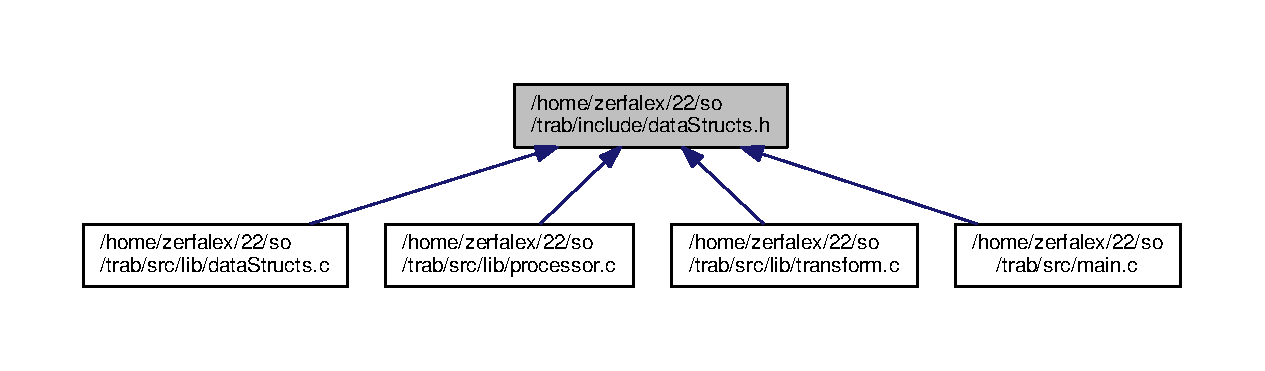
\includegraphics[width=350pt]{data_structs_8h__dep__incl}
\end{center}
\end{figure}
\subsection*{Typedefs}
\begin{DoxyCompactItemize}
\item 
typedef struct \hyperlink{structlist}{list} $\ast$ \hyperlink{data_structs_8h_ad11d86946c524c55becf6a82d77156c1}{L\+I\+ST}
\item 
typedef struct \hyperlink{structthing}{thing} $\ast$ \hyperlink{data_structs_8h_a0c5c1f9da745127fb1a3ca0ce838f645}{T\+H\+I\+NG}
\end{DoxyCompactItemize}
\subsection*{Functions}
\begin{DoxyCompactItemize}
\item 
\hyperlink{data_structs_8h_a0c5c1f9da745127fb1a3ca0ce838f645}{T\+H\+I\+NG} \hyperlink{data_structs_8h_a69b36b99caa22122502147561331ff95}{list\+\_\+get\+\_\+thing} (\hyperlink{data_structs_8h_ad11d86946c524c55becf6a82d77156c1}{L\+I\+ST} l, int index)
\item 
void \hyperlink{data_structs_8h_aea1a0c6f45a8d86668d598afe9ea7012}{list\+\_\+set\+\_\+thing\+\_\+output} (\hyperlink{data_structs_8h_ad11d86946c524c55becf6a82d77156c1}{L\+I\+ST} l, int index, char $\ast$output)
\item 
int \hyperlink{data_structs_8h_a3a6534dc978fbe17afa9b961961b2a8e}{thing\+\_\+get\+\_\+ref} (\hyperlink{data_structs_8h_a0c5c1f9da745127fb1a3ca0ce838f645}{T\+H\+I\+NG} t)
\item 
char $\ast$ \hyperlink{data_structs_8h_ad59f54180d452468db0789d533468e24}{thing\+\_\+get\+\_\+params} (\hyperlink{data_structs_8h_a0c5c1f9da745127fb1a3ca0ce838f645}{T\+H\+I\+NG} t)
\item 
char $\ast$ \hyperlink{data_structs_8h_aa030d07d44f42c1d7e82179b43117941}{thing\+\_\+get\+\_\+output} (\hyperlink{data_structs_8h_a0c5c1f9da745127fb1a3ca0ce838f645}{T\+H\+I\+NG} t)
\item 
int \hyperlink{data_structs_8h_a126b4a3a22c17fe9f61de68ded139f6f}{list\+\_\+size} (\hyperlink{data_structs_8h_ad11d86946c524c55becf6a82d77156c1}{L\+I\+ST} l)
\item 
\hyperlink{data_structs_8h_ad11d86946c524c55becf6a82d77156c1}{L\+I\+ST} \hyperlink{data_structs_8h_ab54221d594955d139687bad10cd269db}{list\+\_\+new} ()
\item 
\hyperlink{data_structs_8h_ad11d86946c524c55becf6a82d77156c1}{L\+I\+ST} \hyperlink{data_structs_8h_a2b902e584b100be6e456738ef6045a8c}{example} ()
\item 
\hyperlink{data_structs_8h_ad11d86946c524c55becf6a82d77156c1}{L\+I\+ST} \hyperlink{data_structs_8h_a8c2ac2ffa00a35e94c3128857bb66616}{list\+\_\+load} (\hyperlink{data_structs_8h_ad11d86946c524c55becf6a82d77156c1}{L\+I\+ST} l, char $\ast$dump)
\item 
void \hyperlink{data_structs_8h_a30a5e7cd4343bebd0fd8e24fb0d0a0f1}{list\+\_\+free} (\hyperlink{data_structs_8h_ad11d86946c524c55becf6a82d77156c1}{L\+I\+ST} l)
\item 
void \hyperlink{data_structs_8h_ae1a3968e7947464bee7714f6d43b7002}{test} ()
\item 
void \hyperlink{data_structs_8h_a3451d9d2f0667d23b8a933cbfc0bf945}{list\+\_\+print} (\hyperlink{data_structs_8h_ad11d86946c524c55becf6a82d77156c1}{L\+I\+ST} l)
\item 
void \hyperlink{data_structs_8h_a70d5833eb5fff25fba4e34920a2eebae}{list\+\_\+add} (\hyperlink{data_structs_8h_ad11d86946c524c55becf6a82d77156c1}{L\+I\+ST} l, int ref, char $\ast$params, char $\ast$output, int sline)
\end{DoxyCompactItemize}


\subsection{Typedef Documentation}
\index{data\+Structs.\+h@{data\+Structs.\+h}!L\+I\+ST@{L\+I\+ST}}
\index{L\+I\+ST@{L\+I\+ST}!data\+Structs.\+h@{data\+Structs.\+h}}
\subsubsection[{\texorpdfstring{L\+I\+ST}{LIST}}]{\setlength{\rightskip}{0pt plus 5cm}typedef struct {\bf list}$\ast$ {\bf L\+I\+ST}}\hypertarget{data_structs_8h_ad11d86946c524c55becf6a82d77156c1}{}\label{data_structs_8h_ad11d86946c524c55becf6a82d77156c1}


Definition at line 4 of file data\+Structs.\+h.

\index{data\+Structs.\+h@{data\+Structs.\+h}!T\+H\+I\+NG@{T\+H\+I\+NG}}
\index{T\+H\+I\+NG@{T\+H\+I\+NG}!data\+Structs.\+h@{data\+Structs.\+h}}
\subsubsection[{\texorpdfstring{T\+H\+I\+NG}{THING}}]{\setlength{\rightskip}{0pt plus 5cm}typedef struct {\bf thing}$\ast$ {\bf T\+H\+I\+NG}}\hypertarget{data_structs_8h_a0c5c1f9da745127fb1a3ca0ce838f645}{}\label{data_structs_8h_a0c5c1f9da745127fb1a3ca0ce838f645}


Definition at line 5 of file data\+Structs.\+h.



\subsection{Function Documentation}
\index{data\+Structs.\+h@{data\+Structs.\+h}!example@{example}}
\index{example@{example}!data\+Structs.\+h@{data\+Structs.\+h}}
\subsubsection[{\texorpdfstring{example()}{example()}}]{\setlength{\rightskip}{0pt plus 5cm}{\bf L\+I\+ST} example (
\begin{DoxyParamCaption}
{}
\end{DoxyParamCaption}
)}\hypertarget{data_structs_8h_a2b902e584b100be6e456738ef6045a8c}{}\label{data_structs_8h_a2b902e584b100be6e456738ef6045a8c}
\index{data\+Structs.\+h@{data\+Structs.\+h}!list\+\_\+add@{list\+\_\+add}}
\index{list\+\_\+add@{list\+\_\+add}!data\+Structs.\+h@{data\+Structs.\+h}}
\subsubsection[{\texorpdfstring{list\+\_\+add(\+L\+I\+S\+T l, int ref, char $\ast$params, char $\ast$output, int sline)}{list_add(LIST l, int ref, char *params, char *output, int sline)}}]{\setlength{\rightskip}{0pt plus 5cm}void list\+\_\+add (
\begin{DoxyParamCaption}
\item[{{\bf L\+I\+ST}}]{l, }
\item[{int}]{ref, }
\item[{char $\ast$}]{params, }
\item[{char $\ast$}]{output, }
\item[{int}]{sline}
\end{DoxyParamCaption}
)}\hypertarget{data_structs_8h_a70d5833eb5fff25fba4e34920a2eebae}{}\label{data_structs_8h_a70d5833eb5fff25fba4e34920a2eebae}
Adds an element to the list with thing\+\_\+new\char`\"{}(\char`\"{}int ref, char $\ast$ params, char $\ast$ output, int sline\char`\"{})\char`\"{}" 
\begin{DoxyParams}{Parameters}
{\em l} & target list \\
\hline
{\em ref} & how many steps back the desired output is \\
\hline
{\em params} & function parameters \\
\hline
{\em output} & processed output \\
\hline
{\em sline} & is part of line, 0 if head of line \\
\hline
\end{DoxyParams}


Definition at line 118 of file data\+Structs.\+c.

\index{data\+Structs.\+h@{data\+Structs.\+h}!list\+\_\+free@{list\+\_\+free}}
\index{list\+\_\+free@{list\+\_\+free}!data\+Structs.\+h@{data\+Structs.\+h}}
\subsubsection[{\texorpdfstring{list\+\_\+free(\+L\+I\+S\+T l)}{list_free(LIST l)}}]{\setlength{\rightskip}{0pt plus 5cm}void list\+\_\+free (
\begin{DoxyParamCaption}
\item[{{\bf L\+I\+ST}}]{l}
\end{DoxyParamCaption}
)}\hypertarget{data_structs_8h_a30a5e7cd4343bebd0fd8e24fb0d0a0f1}{}\label{data_structs_8h_a30a5e7cd4343bebd0fd8e24fb0d0a0f1}
Frees a list\textquotesingle{}s memory allocation 
\begin{DoxyParams}{Parameters}
{\em l} & \mbox{[}description\mbox{]} \\
\hline
\end{DoxyParams}


Definition at line 168 of file data\+Structs.\+c.

\index{data\+Structs.\+h@{data\+Structs.\+h}!list\+\_\+get\+\_\+thing@{list\+\_\+get\+\_\+thing}}
\index{list\+\_\+get\+\_\+thing@{list\+\_\+get\+\_\+thing}!data\+Structs.\+h@{data\+Structs.\+h}}
\subsubsection[{\texorpdfstring{list\+\_\+get\+\_\+thing(\+L\+I\+S\+T l, int index)}{list_get_thing(LIST l, int index)}}]{\setlength{\rightskip}{0pt plus 5cm}{\bf T\+H\+I\+NG} list\+\_\+get\+\_\+thing (
\begin{DoxyParamCaption}
\item[{{\bf L\+I\+ST}}]{l, }
\item[{int}]{index}
\end{DoxyParamCaption}
)}\hypertarget{data_structs_8h_a69b36b99caa22122502147561331ff95}{}\label{data_structs_8h_a69b36b99caa22122502147561331ff95}
Gets a thing from list from position 
\begin{DoxyParams}{Parameters}
{\em l} & a list pointer \\
\hline
{\em index} & position index \\
\hline
\end{DoxyParams}
\begin{DoxyReturn}{Returns}
a thing from the list /note Assumes the caller won\textquotesingle{}t acess beyond the size 
\end{DoxyReturn}


Definition at line 139 of file data\+Structs.\+c.

\index{data\+Structs.\+h@{data\+Structs.\+h}!list\+\_\+load@{list\+\_\+load}}
\index{list\+\_\+load@{list\+\_\+load}!data\+Structs.\+h@{data\+Structs.\+h}}
\subsubsection[{\texorpdfstring{list\+\_\+load(\+L\+I\+S\+T l, char $\ast$dump)}{list_load(LIST l, char *dump)}}]{\setlength{\rightskip}{0pt plus 5cm}{\bf L\+I\+ST} list\+\_\+load (
\begin{DoxyParamCaption}
\item[{{\bf L\+I\+ST}}]{l, }
\item[{char $\ast$}]{dump}
\end{DoxyParamCaption}
)}\hypertarget{data_structs_8h_a8c2ac2ffa00a35e94c3128857bb66616}{}\label{data_structs_8h_a8c2ac2ffa00a35e94c3128857bb66616}
\index{data\+Structs.\+h@{data\+Structs.\+h}!list\+\_\+new@{list\+\_\+new}}
\index{list\+\_\+new@{list\+\_\+new}!data\+Structs.\+h@{data\+Structs.\+h}}
\subsubsection[{\texorpdfstring{list\+\_\+new()}{list_new()}}]{\setlength{\rightskip}{0pt plus 5cm}{\bf L\+I\+ST} list\+\_\+new (
\begin{DoxyParamCaption}
{}
\end{DoxyParamCaption}
)}\hypertarget{data_structs_8h_ab54221d594955d139687bad10cd269db}{}\label{data_structs_8h_ab54221d594955d139687bad10cd269db}
Creates a new, empty list \begin{DoxyReturn}{Returns}
an empty list 
\end{DoxyReturn}


Definition at line 103 of file data\+Structs.\+c.

\index{data\+Structs.\+h@{data\+Structs.\+h}!list\+\_\+print@{list\+\_\+print}}
\index{list\+\_\+print@{list\+\_\+print}!data\+Structs.\+h@{data\+Structs.\+h}}
\subsubsection[{\texorpdfstring{list\+\_\+print(\+L\+I\+S\+T l)}{list_print(LIST l)}}]{\setlength{\rightskip}{0pt plus 5cm}void list\+\_\+print (
\begin{DoxyParamCaption}
\item[{{\bf L\+I\+ST}}]{l}
\end{DoxyParamCaption}
)}\hypertarget{data_structs_8h_a3451d9d2f0667d23b8a933cbfc0bf945}{}\label{data_structs_8h_a3451d9d2f0667d23b8a933cbfc0bf945}
Prints a list by calling void thing\+\_\+print\char`\"{}(\char`\"{}gpointer data, gpointer user\+\_\+data\char`\"{})\char`\"{} on every member of list 
\begin{DoxyParams}{Parameters}
{\em l} & a pointer to a list \\
\hline
\end{DoxyParams}


Definition at line 159 of file data\+Structs.\+c.

\index{data\+Structs.\+h@{data\+Structs.\+h}!list\+\_\+set\+\_\+thing\+\_\+output@{list\+\_\+set\+\_\+thing\+\_\+output}}
\index{list\+\_\+set\+\_\+thing\+\_\+output@{list\+\_\+set\+\_\+thing\+\_\+output}!data\+Structs.\+h@{data\+Structs.\+h}}
\subsubsection[{\texorpdfstring{list\+\_\+set\+\_\+thing\+\_\+output(\+L\+I\+S\+T l, int index, char $\ast$output)}{list_set_thing_output(LIST l, int index, char *output)}}]{\setlength{\rightskip}{0pt plus 5cm}void list\+\_\+set\+\_\+thing\+\_\+output (
\begin{DoxyParamCaption}
\item[{{\bf L\+I\+ST}}]{l, }
\item[{int}]{index, }
\item[{char $\ast$}]{output}
\end{DoxyParamCaption}
)}\hypertarget{data_structs_8h_aea1a0c6f45a8d86668d598afe9ea7012}{}\label{data_structs_8h_aea1a0c6f45a8d86668d598afe9ea7012}
Changes a thing\textquotesingle{}s output given it\textquotesingle{}s position on the list 
\begin{DoxyParams}{Parameters}
{\em l} & a list pointer \\
\hline
{\em index} & position index \\
\hline
{\em output} & a pointer to a thing or N\+U\+LL if it doesn\textquotesingle{}t exist \\
\hline
\end{DoxyParams}


Definition at line 150 of file data\+Structs.\+c.

\index{data\+Structs.\+h@{data\+Structs.\+h}!list\+\_\+size@{list\+\_\+size}}
\index{list\+\_\+size@{list\+\_\+size}!data\+Structs.\+h@{data\+Structs.\+h}}
\subsubsection[{\texorpdfstring{list\+\_\+size(\+L\+I\+S\+T l)}{list_size(LIST l)}}]{\setlength{\rightskip}{0pt plus 5cm}int list\+\_\+size (
\begin{DoxyParamCaption}
\item[{{\bf L\+I\+ST}}]{l}
\end{DoxyParamCaption}
)}\hypertarget{data_structs_8h_a126b4a3a22c17fe9f61de68ded139f6f}{}\label{data_structs_8h_a126b4a3a22c17fe9f61de68ded139f6f}
Returns a list\textquotesingle{}s size 
\begin{DoxyParams}{Parameters}
{\em l} & a list pointer \\
\hline
\end{DoxyParams}
\begin{DoxyReturn}{Returns}
list size 
\end{DoxyReturn}


Definition at line 128 of file data\+Structs.\+c.

\index{data\+Structs.\+h@{data\+Structs.\+h}!test@{test}}
\index{test@{test}!data\+Structs.\+h@{data\+Structs.\+h}}
\subsubsection[{\texorpdfstring{test()}{test()}}]{\setlength{\rightskip}{0pt plus 5cm}void test (
\begin{DoxyParamCaption}
{}
\end{DoxyParamCaption}
)}\hypertarget{data_structs_8h_ae1a3968e7947464bee7714f6d43b7002}{}\label{data_structs_8h_ae1a3968e7947464bee7714f6d43b7002}
\index{data\+Structs.\+h@{data\+Structs.\+h}!thing\+\_\+get\+\_\+output@{thing\+\_\+get\+\_\+output}}
\index{thing\+\_\+get\+\_\+output@{thing\+\_\+get\+\_\+output}!data\+Structs.\+h@{data\+Structs.\+h}}
\subsubsection[{\texorpdfstring{thing\+\_\+get\+\_\+output(\+T\+H\+I\+N\+G t)}{thing_get_output(THING t)}}]{\setlength{\rightskip}{0pt plus 5cm}char$\ast$ thing\+\_\+get\+\_\+output (
\begin{DoxyParamCaption}
\item[{{\bf T\+H\+I\+NG}}]{t}
\end{DoxyParamCaption}
)}\hypertarget{data_structs_8h_aa030d07d44f42c1d7e82179b43117941}{}\label{data_structs_8h_aa030d07d44f42c1d7e82179b43117941}
Returns a t\textquotesingle{}s parameters 
\begin{DoxyParams}{Parameters}
{\em t} & a pointer to the thing \\
\hline
\end{DoxyParams}
\begin{DoxyReturn}{Returns}
a string with the output 
\end{DoxyReturn}


Definition at line 72 of file data\+Structs.\+c.

\index{data\+Structs.\+h@{data\+Structs.\+h}!thing\+\_\+get\+\_\+params@{thing\+\_\+get\+\_\+params}}
\index{thing\+\_\+get\+\_\+params@{thing\+\_\+get\+\_\+params}!data\+Structs.\+h@{data\+Structs.\+h}}
\subsubsection[{\texorpdfstring{thing\+\_\+get\+\_\+params(\+T\+H\+I\+N\+G t)}{thing_get_params(THING t)}}]{\setlength{\rightskip}{0pt plus 5cm}char$\ast$ thing\+\_\+get\+\_\+params (
\begin{DoxyParamCaption}
\item[{{\bf T\+H\+I\+NG}}]{t}
\end{DoxyParamCaption}
)}\hypertarget{data_structs_8h_ad59f54180d452468db0789d533468e24}{}\label{data_structs_8h_ad59f54180d452468db0789d533468e24}
Returns a t\textquotesingle{}s parameters 
\begin{DoxyParams}{Parameters}
{\em t} & a pointer to the thing \\
\hline
\end{DoxyParams}
\begin{DoxyReturn}{Returns}
a string with parameters 
\end{DoxyReturn}


Definition at line 62 of file data\+Structs.\+c.

\index{data\+Structs.\+h@{data\+Structs.\+h}!thing\+\_\+get\+\_\+ref@{thing\+\_\+get\+\_\+ref}}
\index{thing\+\_\+get\+\_\+ref@{thing\+\_\+get\+\_\+ref}!data\+Structs.\+h@{data\+Structs.\+h}}
\subsubsection[{\texorpdfstring{thing\+\_\+get\+\_\+ref(\+T\+H\+I\+N\+G t)}{thing_get_ref(THING t)}}]{\setlength{\rightskip}{0pt plus 5cm}int thing\+\_\+get\+\_\+ref (
\begin{DoxyParamCaption}
\item[{{\bf T\+H\+I\+NG}}]{t}
\end{DoxyParamCaption}
)}\hypertarget{data_structs_8h_a3a6534dc978fbe17afa9b961961b2a8e}{}\label{data_structs_8h_a3a6534dc978fbe17afa9b961961b2a8e}
Returns a t\textquotesingle{}s reference nummber 
\begin{DoxyParams}{Parameters}
{\em t} & a pointer to the thing \\
\hline
\end{DoxyParams}
\begin{DoxyReturn}{Returns}
a reference number 
\end{DoxyReturn}


Definition at line 53 of file data\+Structs.\+c.


\hypertarget{processor_8h}{}\section{/home/zerfalex/22/so/trab/include/processor.h File Reference}
\label{processor_8h}\index{/home/zerfalex/22/so/trab/include/processor.\+h@{/home/zerfalex/22/so/trab/include/processor.\+h}}
This graph shows which files directly or indirectly include this file\+:\nopagebreak
\begin{figure}[H]
\begin{center}
\leavevmode
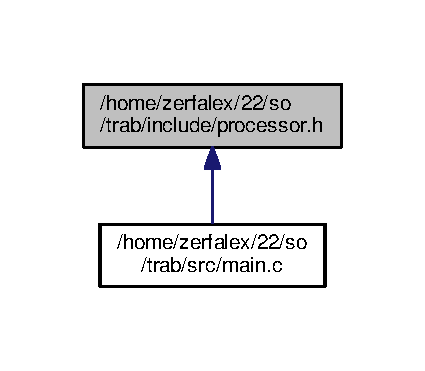
\includegraphics[width=204pt]{processor_8h__dep__incl}
\end{center}
\end{figure}
\subsection*{Functions}
\begin{DoxyCompactItemize}
\item 
int \hyperlink{processor_8h_a73841513cc2eb16fe26b634e28755580}{list\+\_\+process} (\hyperlink{data_structs_8h_a02dfe73aee9a117ed44a7abc305f1066}{L\+I\+ST} l)
\end{DoxyCompactItemize}


\subsection{Function Documentation}
\index{processor.\+h@{processor.\+h}!list\+\_\+process@{list\+\_\+process}}
\index{list\+\_\+process@{list\+\_\+process}!processor.\+h@{processor.\+h}}
\subsubsection[{\texorpdfstring{list\+\_\+process(\+L\+I\+S\+T l)}{list_process(LIST l)}}]{\setlength{\rightskip}{0pt plus 5cm}int list\+\_\+process (
\begin{DoxyParamCaption}
\item[{{\bf L\+I\+ST}}]{list}
\end{DoxyParamCaption}
)}\hypertarget{processor_8h_a73841513cc2eb16fe26b634e28755580}{}\label{processor_8h_a73841513cc2eb16fe26b634e28755580}
Processes l, fillin all output fields 
\begin{DoxyParams}{Parameters}
{\em l} & a L\+I\+ST \\
\hline
\end{DoxyParams}
\begin{DoxyReturn}{Returns}
and int indicating how the process went /note hello 
\end{DoxyReturn}


Definition at line 26 of file processor.\+c.


\hypertarget{transform_8h}{}\section{/home/zerfalex/22/so/trab/include/transform.h File Reference}
\label{transform_8h}\index{/home/zerfalex/22/so/trab/include/transform.\+h@{/home/zerfalex/22/so/trab/include/transform.\+h}}
This graph shows which files directly or indirectly include this file\+:\nopagebreak
\begin{figure}[H]
\begin{center}
\leavevmode
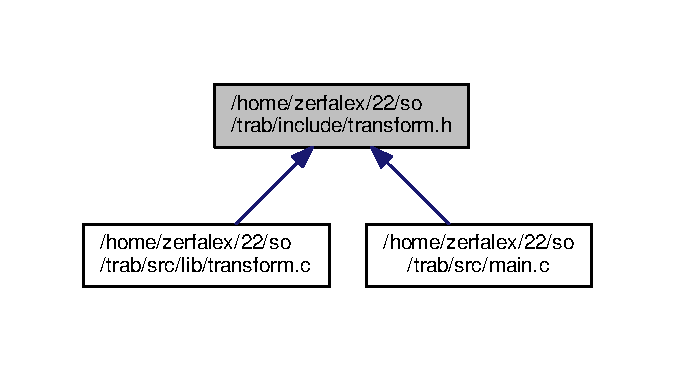
\includegraphics[width=324pt]{transform_8h__dep__incl}
\end{center}
\end{figure}
\subsection*{Functions}
\begin{DoxyCompactItemize}
\item 
void \hyperlink{transform_8h_a41104cfc27eb72adf15afc72b19fc705}{note\+To\+List} (int argc, char $\ast$argv\mbox{[}$\,$\mbox{]}, \hyperlink{data_structs_8h_a02dfe73aee9a117ed44a7abc305f1066}{L\+I\+ST} \hyperlink{structlist}{list})
\item 
void \hyperlink{transform_8h_ac700a91d14c71a5f71c4793ecbfee12d}{list\+To\+Note} (int argc, char $\ast$argv\mbox{[}$\,$\mbox{]}, \hyperlink{data_structs_8h_a02dfe73aee9a117ed44a7abc305f1066}{L\+I\+ST} \hyperlink{structlist}{list})
\end{DoxyCompactItemize}


\subsection{Function Documentation}
\index{transform.\+h@{transform.\+h}!list\+To\+Note@{list\+To\+Note}}
\index{list\+To\+Note@{list\+To\+Note}!transform.\+h@{transform.\+h}}
\subsubsection[{\texorpdfstring{list\+To\+Note(int argc, char $\ast$argv[], L\+I\+S\+T list)}{listToNote(int argc, char *argv[], LIST list)}}]{\setlength{\rightskip}{0pt plus 5cm}void list\+To\+Note (
\begin{DoxyParamCaption}
\item[{int}]{argc, }
\item[{char $\ast$}]{argv\mbox{[}$\,$\mbox{]}, }
\item[{{\bf L\+I\+ST}}]{list}
\end{DoxyParamCaption}
)}\hypertarget{transform_8h_ac700a91d14c71a5f71c4793ecbfee12d}{}\label{transform_8h_ac700a91d14c71a5f71c4793ecbfee12d}


Definition at line 32 of file transform.\+c.

\index{transform.\+h@{transform.\+h}!note\+To\+List@{note\+To\+List}}
\index{note\+To\+List@{note\+To\+List}!transform.\+h@{transform.\+h}}
\subsubsection[{\texorpdfstring{note\+To\+List(int argc, char $\ast$argv[], L\+I\+S\+T list)}{noteToList(int argc, char *argv[], LIST list)}}]{\setlength{\rightskip}{0pt plus 5cm}void note\+To\+List (
\begin{DoxyParamCaption}
\item[{int}]{argc, }
\item[{char $\ast$}]{argv\mbox{[}$\,$\mbox{]}, }
\item[{{\bf L\+I\+ST}}]{list}
\end{DoxyParamCaption}
)}\hypertarget{transform_8h_a41104cfc27eb72adf15afc72b19fc705}{}\label{transform_8h_a41104cfc27eb72adf15afc72b19fc705}


Definition at line 12 of file transform.\+c.


\hypertarget{data_structs_8c}{}\section{/home/zerfalex/22/so/trab/src/lib/data\+Structs.c File Reference}
\label{data_structs_8c}\index{/home/zerfalex/22/so/trab/src/lib/data\+Structs.\+c@{/home/zerfalex/22/so/trab/src/lib/data\+Structs.\+c}}
{\ttfamily \#include $<$stdlib.\+h$>$}\\*
{\ttfamily \#include $<$gmodule.\+h$>$}\\*
{\ttfamily \#include $<$string.\+h$>$}\\*
{\ttfamily \#include $<$unistd.\+h$>$}\\*
{\ttfamily \#include $<$stdio.\+h$>$}\\*
{\ttfamily \#include $<$stdint.\+h$>$}\\*
{\ttfamily \#include $<$data\+Structs.\+h$>$}\\*
Include dependency graph for data\+Structs.\+c\+:\nopagebreak
\begin{figure}[H]
\begin{center}
\leavevmode
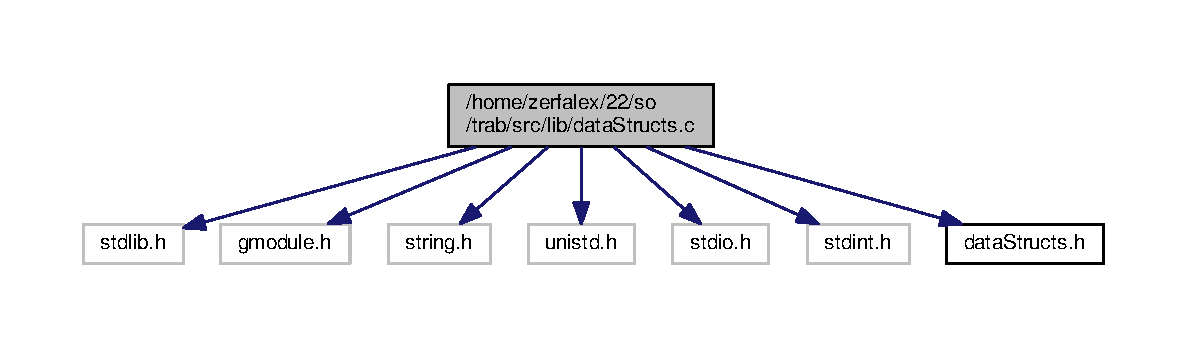
\includegraphics[width=350pt]{data_structs_8c__incl}
\end{center}
\end{figure}
\subsection*{Data Structures}
\begin{DoxyCompactItemize}
\item 
struct \hyperlink{structlist}{list}
\begin{DoxyCompactList}\small\item\em A list containing a G\+Ptr\+Array and an int for size. \end{DoxyCompactList}\item 
struct \hyperlink{structthing}{thing}
\begin{DoxyCompactList}\small\item\em A struct which houses a command\textquotesingle{}s parameters, it\textquotesingle{}s, if parsed, output, reference and sline value. \end{DoxyCompactList}\end{DoxyCompactItemize}
\subsection*{Functions}
\begin{DoxyCompactItemize}
\item 
\hyperlink{data_structs_8h_aa715de5e15fcce8d01aa142936095a38}{T\+H\+I\+NG} \hyperlink{data_structs_8c_a5c1a6bff74782d4314539fc728dceb7c}{thing\+\_\+new} (int ref, char $\ast$params, char $\ast$output, int sline)
\item 
int \hyperlink{data_structs_8c_a3a6534dc978fbe17afa9b961961b2a8e}{thing\+\_\+get\+\_\+ref} (\hyperlink{data_structs_8h_aa715de5e15fcce8d01aa142936095a38}{T\+H\+I\+NG} t)
\item 
int \hyperlink{data_structs_8c_ae140b76dc86dc5a8cf50e3a56f6f2ef1}{thing\+\_\+get\+\_\+sline} (\hyperlink{data_structs_8h_aa715de5e15fcce8d01aa142936095a38}{T\+H\+I\+NG} t)
\item 
char $\ast$ \hyperlink{data_structs_8c_ad59f54180d452468db0789d533468e24}{thing\+\_\+get\+\_\+params} (\hyperlink{data_structs_8h_aa715de5e15fcce8d01aa142936095a38}{T\+H\+I\+NG} t)
\item 
char $\ast$ \hyperlink{data_structs_8c_aa030d07d44f42c1d7e82179b43117941}{thing\+\_\+get\+\_\+output} (\hyperlink{data_structs_8h_aa715de5e15fcce8d01aa142936095a38}{T\+H\+I\+NG} t)
\item 
void \hyperlink{data_structs_8c_a2d5cf1f668dadd619a6adafdbc88c027}{thing\+\_\+free} (gpointer data)
\item 
void \hyperlink{data_structs_8c_a7071db3198cf59e3b5eb5c4f9b87636c}{thing\+\_\+print} (gpointer data, gpointer user\+\_\+data)
\item 
\hyperlink{data_structs_8h_a02dfe73aee9a117ed44a7abc305f1066}{L\+I\+ST} \hyperlink{data_structs_8c_ab54221d594955d139687bad10cd269db}{list\+\_\+new} ()
\item 
void \hyperlink{data_structs_8c_a70d5833eb5fff25fba4e34920a2eebae}{list\+\_\+add} (\hyperlink{data_structs_8h_a02dfe73aee9a117ed44a7abc305f1066}{L\+I\+ST} l, int ref, char $\ast$params, char $\ast$output, int sline)
\item 
int \hyperlink{data_structs_8c_a126b4a3a22c17fe9f61de68ded139f6f}{list\+\_\+size} (\hyperlink{data_structs_8h_a02dfe73aee9a117ed44a7abc305f1066}{L\+I\+ST} l)
\item 
\hyperlink{data_structs_8h_aa715de5e15fcce8d01aa142936095a38}{T\+H\+I\+NG} \hyperlink{data_structs_8c_a69b36b99caa22122502147561331ff95}{list\+\_\+get\+\_\+thing} (\hyperlink{data_structs_8h_a02dfe73aee9a117ed44a7abc305f1066}{L\+I\+ST} l, int index)
\item 
void \hyperlink{data_structs_8c_aea1a0c6f45a8d86668d598afe9ea7012}{list\+\_\+set\+\_\+thing\+\_\+output} (\hyperlink{data_structs_8h_a02dfe73aee9a117ed44a7abc305f1066}{L\+I\+ST} l, int index, char $\ast$output)
\item 
void \hyperlink{data_structs_8c_a3451d9d2f0667d23b8a933cbfc0bf945}{list\+\_\+print} (\hyperlink{data_structs_8h_a02dfe73aee9a117ed44a7abc305f1066}{L\+I\+ST} l)
\item 
void \hyperlink{data_structs_8c_a30a5e7cd4343bebd0fd8e24fb0d0a0f1}{list\+\_\+free} (\hyperlink{data_structs_8h_a02dfe73aee9a117ed44a7abc305f1066}{L\+I\+ST} l)
\end{DoxyCompactItemize}


\subsection{Function Documentation}
\index{data\+Structs.\+c@{data\+Structs.\+c}!list\+\_\+add@{list\+\_\+add}}
\index{list\+\_\+add@{list\+\_\+add}!data\+Structs.\+c@{data\+Structs.\+c}}
\subsubsection[{\texorpdfstring{list\+\_\+add(\+L\+I\+S\+T l, int ref, char $\ast$params, char $\ast$output, int sline)}{list_add(LIST l, int ref, char *params, char *output, int sline)}}]{\setlength{\rightskip}{0pt plus 5cm}void list\+\_\+add (
\begin{DoxyParamCaption}
\item[{{\bf L\+I\+ST}}]{l, }
\item[{int}]{ref, }
\item[{char $\ast$}]{params, }
\item[{char $\ast$}]{output, }
\item[{int}]{sline}
\end{DoxyParamCaption}
)}\hypertarget{data_structs_8c_a70d5833eb5fff25fba4e34920a2eebae}{}\label{data_structs_8c_a70d5833eb5fff25fba4e34920a2eebae}
Adds an element to the list with thing\+\_\+new\char`\"{}(\char`\"{}int ref, char $\ast$ params, char $\ast$ output, int sline\char`\"{})\char`\"{}" 
\begin{DoxyParams}{Parameters}
{\em l} & target list \\
\hline
{\em ref} & how many steps back the desired output is \\
\hline
{\em params} & function parameters \\
\hline
{\em output} & processed output \\
\hline
{\em sline} & is part of line, 0 if head of line \\
\hline
\end{DoxyParams}


Definition at line 136 of file data\+Structs.\+c.

\index{data\+Structs.\+c@{data\+Structs.\+c}!list\+\_\+free@{list\+\_\+free}}
\index{list\+\_\+free@{list\+\_\+free}!data\+Structs.\+c@{data\+Structs.\+c}}
\subsubsection[{\texorpdfstring{list\+\_\+free(\+L\+I\+S\+T l)}{list_free(LIST l)}}]{\setlength{\rightskip}{0pt plus 5cm}void list\+\_\+free (
\begin{DoxyParamCaption}
\item[{{\bf L\+I\+ST}}]{l}
\end{DoxyParamCaption}
)}\hypertarget{data_structs_8c_a30a5e7cd4343bebd0fd8e24fb0d0a0f1}{}\label{data_structs_8c_a30a5e7cd4343bebd0fd8e24fb0d0a0f1}
Frees a list\textquotesingle{}s memory allocation 
\begin{DoxyParams}{Parameters}
{\em l} & \mbox{[}description\mbox{]} \\
\hline
\end{DoxyParams}


Definition at line 186 of file data\+Structs.\+c.

\index{data\+Structs.\+c@{data\+Structs.\+c}!list\+\_\+get\+\_\+thing@{list\+\_\+get\+\_\+thing}}
\index{list\+\_\+get\+\_\+thing@{list\+\_\+get\+\_\+thing}!data\+Structs.\+c@{data\+Structs.\+c}}
\subsubsection[{\texorpdfstring{list\+\_\+get\+\_\+thing(\+L\+I\+S\+T l, int index)}{list_get_thing(LIST l, int index)}}]{\setlength{\rightskip}{0pt plus 5cm}{\bf T\+H\+I\+NG} list\+\_\+get\+\_\+thing (
\begin{DoxyParamCaption}
\item[{{\bf L\+I\+ST}}]{l, }
\item[{int}]{index}
\end{DoxyParamCaption}
)}\hypertarget{data_structs_8c_a69b36b99caa22122502147561331ff95}{}\label{data_structs_8c_a69b36b99caa22122502147561331ff95}
Gets a thing from list from position 
\begin{DoxyParams}{Parameters}
{\em l} & a list pointer \\
\hline
{\em index} & position index \\
\hline
\end{DoxyParams}
\begin{DoxyReturn}{Returns}
a thing from the list /note Assumes the caller won\textquotesingle{}t acess beyond the size 
\end{DoxyReturn}


Definition at line 157 of file data\+Structs.\+c.

\index{data\+Structs.\+c@{data\+Structs.\+c}!list\+\_\+new@{list\+\_\+new}}
\index{list\+\_\+new@{list\+\_\+new}!data\+Structs.\+c@{data\+Structs.\+c}}
\subsubsection[{\texorpdfstring{list\+\_\+new()}{list_new()}}]{\setlength{\rightskip}{0pt plus 5cm}{\bf L\+I\+ST} list\+\_\+new (
\begin{DoxyParamCaption}
{}
\end{DoxyParamCaption}
)}\hypertarget{data_structs_8c_ab54221d594955d139687bad10cd269db}{}\label{data_structs_8c_ab54221d594955d139687bad10cd269db}
Creates a new, empty list \begin{DoxyReturn}{Returns}
an empty list 
\end{DoxyReturn}


Definition at line 121 of file data\+Structs.\+c.

\index{data\+Structs.\+c@{data\+Structs.\+c}!list\+\_\+print@{list\+\_\+print}}
\index{list\+\_\+print@{list\+\_\+print}!data\+Structs.\+c@{data\+Structs.\+c}}
\subsubsection[{\texorpdfstring{list\+\_\+print(\+L\+I\+S\+T l)}{list_print(LIST l)}}]{\setlength{\rightskip}{0pt plus 5cm}void list\+\_\+print (
\begin{DoxyParamCaption}
\item[{{\bf L\+I\+ST}}]{l}
\end{DoxyParamCaption}
)}\hypertarget{data_structs_8c_a3451d9d2f0667d23b8a933cbfc0bf945}{}\label{data_structs_8c_a3451d9d2f0667d23b8a933cbfc0bf945}
Prints a list by calling void thing\+\_\+print\char`\"{}(\char`\"{}gpointer data, gpointer user\+\_\+data\char`\"{})\char`\"{} on every member of list 
\begin{DoxyParams}{Parameters}
{\em l} & a pointer to a list \\
\hline
\end{DoxyParams}


Definition at line 177 of file data\+Structs.\+c.

\index{data\+Structs.\+c@{data\+Structs.\+c}!list\+\_\+set\+\_\+thing\+\_\+output@{list\+\_\+set\+\_\+thing\+\_\+output}}
\index{list\+\_\+set\+\_\+thing\+\_\+output@{list\+\_\+set\+\_\+thing\+\_\+output}!data\+Structs.\+c@{data\+Structs.\+c}}
\subsubsection[{\texorpdfstring{list\+\_\+set\+\_\+thing\+\_\+output(\+L\+I\+S\+T l, int index, char $\ast$output)}{list_set_thing_output(LIST l, int index, char *output)}}]{\setlength{\rightskip}{0pt plus 5cm}void list\+\_\+set\+\_\+thing\+\_\+output (
\begin{DoxyParamCaption}
\item[{{\bf L\+I\+ST}}]{l, }
\item[{int}]{index, }
\item[{char $\ast$}]{output}
\end{DoxyParamCaption}
)}\hypertarget{data_structs_8c_aea1a0c6f45a8d86668d598afe9ea7012}{}\label{data_structs_8c_aea1a0c6f45a8d86668d598afe9ea7012}
Changes a thing\textquotesingle{}s output given it\textquotesingle{}s position on the list 
\begin{DoxyParams}{Parameters}
{\em l} & a list pointer \\
\hline
{\em index} & position index \\
\hline
{\em output} & a pointer to a thing or N\+U\+LL if it doesn\textquotesingle{}t exist \\
\hline
\end{DoxyParams}


Definition at line 168 of file data\+Structs.\+c.

\index{data\+Structs.\+c@{data\+Structs.\+c}!list\+\_\+size@{list\+\_\+size}}
\index{list\+\_\+size@{list\+\_\+size}!data\+Structs.\+c@{data\+Structs.\+c}}
\subsubsection[{\texorpdfstring{list\+\_\+size(\+L\+I\+S\+T l)}{list_size(LIST l)}}]{\setlength{\rightskip}{0pt plus 5cm}int list\+\_\+size (
\begin{DoxyParamCaption}
\item[{{\bf L\+I\+ST}}]{l}
\end{DoxyParamCaption}
)}\hypertarget{data_structs_8c_a126b4a3a22c17fe9f61de68ded139f6f}{}\label{data_structs_8c_a126b4a3a22c17fe9f61de68ded139f6f}
Returns a list\textquotesingle{}s size 
\begin{DoxyParams}{Parameters}
{\em l} & a list pointer \\
\hline
\end{DoxyParams}
\begin{DoxyReturn}{Returns}
list size 
\end{DoxyReturn}


Definition at line 146 of file data\+Structs.\+c.

\index{data\+Structs.\+c@{data\+Structs.\+c}!thing\+\_\+free@{thing\+\_\+free}}
\index{thing\+\_\+free@{thing\+\_\+free}!data\+Structs.\+c@{data\+Structs.\+c}}
\subsubsection[{\texorpdfstring{thing\+\_\+free(gpointer data)}{thing_free(gpointer data)}}]{\setlength{\rightskip}{0pt plus 5cm}void thing\+\_\+free (
\begin{DoxyParamCaption}
\item[{gpointer}]{data}
\end{DoxyParamCaption}
)}\hypertarget{data_structs_8c_a2d5cf1f668dadd619a6adafdbc88c027}{}\label{data_structs_8c_a2d5cf1f668dadd619a6adafdbc88c027}
Frees a thing\textquotesingle{}s memory allocation 
\begin{DoxyParams}{Parameters}
{\em data} & a pointer to the thing \\
\hline
\end{DoxyParams}


Definition at line 100 of file data\+Structs.\+c.

\index{data\+Structs.\+c@{data\+Structs.\+c}!thing\+\_\+get\+\_\+output@{thing\+\_\+get\+\_\+output}}
\index{thing\+\_\+get\+\_\+output@{thing\+\_\+get\+\_\+output}!data\+Structs.\+c@{data\+Structs.\+c}}
\subsubsection[{\texorpdfstring{thing\+\_\+get\+\_\+output(\+T\+H\+I\+N\+G t)}{thing_get_output(THING t)}}]{\setlength{\rightskip}{0pt plus 5cm}char$\ast$ thing\+\_\+get\+\_\+output (
\begin{DoxyParamCaption}
\item[{{\bf T\+H\+I\+NG}}]{t}
\end{DoxyParamCaption}
)}\hypertarget{data_structs_8c_aa030d07d44f42c1d7e82179b43117941}{}\label{data_structs_8c_aa030d07d44f42c1d7e82179b43117941}
Returns a t\textquotesingle{}s parameters 
\begin{DoxyParams}{Parameters}
{\em t} & a pointer to the thing \\
\hline
\end{DoxyParams}
\begin{DoxyReturn}{Returns}
a string with the output 
\end{DoxyReturn}


Definition at line 90 of file data\+Structs.\+c.

\index{data\+Structs.\+c@{data\+Structs.\+c}!thing\+\_\+get\+\_\+params@{thing\+\_\+get\+\_\+params}}
\index{thing\+\_\+get\+\_\+params@{thing\+\_\+get\+\_\+params}!data\+Structs.\+c@{data\+Structs.\+c}}
\subsubsection[{\texorpdfstring{thing\+\_\+get\+\_\+params(\+T\+H\+I\+N\+G t)}{thing_get_params(THING t)}}]{\setlength{\rightskip}{0pt plus 5cm}char$\ast$ thing\+\_\+get\+\_\+params (
\begin{DoxyParamCaption}
\item[{{\bf T\+H\+I\+NG}}]{t}
\end{DoxyParamCaption}
)}\hypertarget{data_structs_8c_ad59f54180d452468db0789d533468e24}{}\label{data_structs_8c_ad59f54180d452468db0789d533468e24}
Returns a t\textquotesingle{}s parameters 
\begin{DoxyParams}{Parameters}
{\em t} & a pointer to the thing \\
\hline
\end{DoxyParams}
\begin{DoxyReturn}{Returns}
a string with parameters 
\end{DoxyReturn}


Definition at line 80 of file data\+Structs.\+c.

\index{data\+Structs.\+c@{data\+Structs.\+c}!thing\+\_\+get\+\_\+ref@{thing\+\_\+get\+\_\+ref}}
\index{thing\+\_\+get\+\_\+ref@{thing\+\_\+get\+\_\+ref}!data\+Structs.\+c@{data\+Structs.\+c}}
\subsubsection[{\texorpdfstring{thing\+\_\+get\+\_\+ref(\+T\+H\+I\+N\+G t)}{thing_get_ref(THING t)}}]{\setlength{\rightskip}{0pt plus 5cm}int thing\+\_\+get\+\_\+ref (
\begin{DoxyParamCaption}
\item[{{\bf T\+H\+I\+NG}}]{t}
\end{DoxyParamCaption}
)}\hypertarget{data_structs_8c_a3a6534dc978fbe17afa9b961961b2a8e}{}\label{data_structs_8c_a3a6534dc978fbe17afa9b961961b2a8e}
Returns a t\textquotesingle{}s reference nummber 
\begin{DoxyParams}{Parameters}
{\em t} & a pointer to the thing \\
\hline
\end{DoxyParams}
\begin{DoxyReturn}{Returns}
a reference number 
\end{DoxyReturn}


Definition at line 62 of file data\+Structs.\+c.

\index{data\+Structs.\+c@{data\+Structs.\+c}!thing\+\_\+get\+\_\+sline@{thing\+\_\+get\+\_\+sline}}
\index{thing\+\_\+get\+\_\+sline@{thing\+\_\+get\+\_\+sline}!data\+Structs.\+c@{data\+Structs.\+c}}
\subsubsection[{\texorpdfstring{thing\+\_\+get\+\_\+sline(\+T\+H\+I\+N\+G t)}{thing_get_sline(THING t)}}]{\setlength{\rightskip}{0pt plus 5cm}int thing\+\_\+get\+\_\+sline (
\begin{DoxyParamCaption}
\item[{{\bf T\+H\+I\+NG}}]{t}
\end{DoxyParamCaption}
)}\hypertarget{data_structs_8c_ae140b76dc86dc5a8cf50e3a56f6f2ef1}{}\label{data_structs_8c_ae140b76dc86dc5a8cf50e3a56f6f2ef1}
Returns a t\textquotesingle{}s sline 
\begin{DoxyParams}{Parameters}
{\em t} & a pointer to the thing \\
\hline
\end{DoxyParams}
\begin{DoxyReturn}{Returns}
a sline number 
\end{DoxyReturn}


Definition at line 71 of file data\+Structs.\+c.

\index{data\+Structs.\+c@{data\+Structs.\+c}!thing\+\_\+new@{thing\+\_\+new}}
\index{thing\+\_\+new@{thing\+\_\+new}!data\+Structs.\+c@{data\+Structs.\+c}}
\subsubsection[{\texorpdfstring{thing\+\_\+new(int ref, char $\ast$params, char $\ast$output, int sline)}{thing_new(int ref, char *params, char *output, int sline)}}]{\setlength{\rightskip}{0pt plus 5cm}{\bf T\+H\+I\+NG} thing\+\_\+new (
\begin{DoxyParamCaption}
\item[{int}]{ref, }
\item[{char $\ast$}]{params, }
\item[{char $\ast$}]{output, }
\item[{int}]{sline}
\end{DoxyParamCaption}
)}\hypertarget{data_structs_8c_a5c1a6bff74782d4314539fc728dceb7c}{}\label{data_structs_8c_a5c1a6bff74782d4314539fc728dceb7c}
Creates a new T\+H\+I\+NG 
\begin{DoxyParams}{Parameters}
{\em ref} & how many steps back the desired output is \\
\hline
{\em params} & function parameters \\
\hline
{\em output} & processed output \\
\hline
{\em sline} & is part of line, 0 if head of line \\
\hline
\end{DoxyParams}
\begin{DoxyReturn}{Returns}
a new T\+H\+I\+NG. 
\end{DoxyReturn}


Definition at line 39 of file data\+Structs.\+c.

\index{data\+Structs.\+c@{data\+Structs.\+c}!thing\+\_\+print@{thing\+\_\+print}}
\index{thing\+\_\+print@{thing\+\_\+print}!data\+Structs.\+c@{data\+Structs.\+c}}
\subsubsection[{\texorpdfstring{thing\+\_\+print(gpointer data, gpointer user\+\_\+data)}{thing_print(gpointer data, gpointer user_data)}}]{\setlength{\rightskip}{0pt plus 5cm}void thing\+\_\+print (
\begin{DoxyParamCaption}
\item[{gpointer}]{data, }
\item[{gpointer}]{user\+\_\+data}
\end{DoxyParamCaption}
)}\hypertarget{data_structs_8c_a7071db3198cf59e3b5eb5c4f9b87636c}{}\label{data_structs_8c_a7071db3198cf59e3b5eb5c4f9b87636c}
Prints out a thing 
\begin{DoxyParams}{Parameters}
{\em data} & thing pointer \\
\hline
{\em user\+\_\+data} & pointer to user passed data \\
\hline
\end{DoxyParams}


Definition at line 112 of file data\+Structs.\+c.


\section{/home/zerfalex/22/so/trab/src/lib/processor.c File Reference}
\label{processor_8c}\index{/home/zerfalex/22/so/trab/src/lib/processor.\+c@{/home/zerfalex/22/so/trab/src/lib/processor.\+c}}
{\ttfamily \#include $<$stdlib.\+h$>$}\\*
{\ttfamily \#include $<$gmodule.\+h$>$}\\*
{\ttfamily \#include $<$string.\+h$>$}\\*
{\ttfamily \#include $<$unistd.\+h$>$}\\*
{\ttfamily \#include $<$stdio.\+h$>$}\\*
{\ttfamily \#include $<$stdint.\+h$>$}\\*
{\ttfamily \#include $<$data\+Structs.\+h$>$}\\*
{\ttfamily \#include $<$sys/types.\+h$>$}\\*
{\ttfamily \#include $<$sys/wait.\+h$>$}\\*
{\ttfamily \#include $<$sys/stat.\+h$>$}\\*
{\ttfamily \#include $<$fcntl.\+h$>$}\\*
{\ttfamily \#include $<$signal.\+h$>$}\\*
Include dependency graph for processor.\+c\+:\nopagebreak
\begin{figure}[H]
\begin{center}
\leavevmode
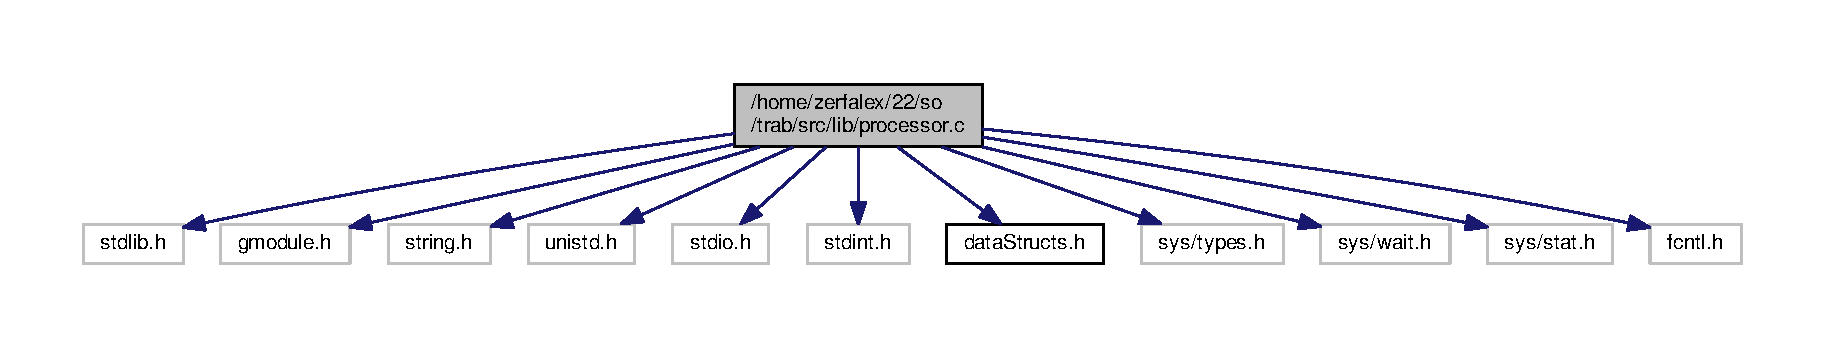
\includegraphics[width=350pt]{processor_8c__incl}
\end{center}
\end{figure}
\subsection*{Typedefs}
\begin{DoxyCompactItemize}
\item 
typedef void($\ast$ {\bf sighandler\+\_\+t}) (int)
\end{DoxyCompactItemize}
\subsection*{Functions}
\begin{DoxyCompactItemize}
\item 
int {\bf list\+\_\+process} ({\bf L\+I\+ST} {\bf list})
\end{DoxyCompactItemize}


\subsection{Typedef Documentation}
\index{processor.\+c@{processor.\+c}!sighandler\+\_\+t@{sighandler\+\_\+t}}
\index{sighandler\+\_\+t@{sighandler\+\_\+t}!processor.\+c@{processor.\+c}}
\subsubsection[{sighandler\+\_\+t}]{\setlength{\rightskip}{0pt plus 5cm}typedef void($\ast$ sighandler\+\_\+t) (int)}\label{processor_8c_a754cdc0bcfffe07baa426dc252c9101a}


Definition at line 18 of file processor.\+c.



\subsection{Function Documentation}
\index{processor.\+c@{processor.\+c}!list\+\_\+process@{list\+\_\+process}}
\index{list\+\_\+process@{list\+\_\+process}!processor.\+c@{processor.\+c}}
\subsubsection[{list\+\_\+process(\+L\+I\+S\+T list)}]{\setlength{\rightskip}{0pt plus 5cm}int list\+\_\+process (
\begin{DoxyParamCaption}
\item[{{\bf L\+I\+ST}}]{list}
\end{DoxyParamCaption}
)}\label{processor_8c_aea6d083cebe2f047861e31facc48ae02}
Processes l, fillin all output fields 
\begin{DoxyParams}{Parameters}
{\em l} & a L\+I\+ST \\
\hline
\end{DoxyParams}
\begin{DoxyReturn}{Returns}
and int indicating how the process went /note hello 
\end{DoxyReturn}


Definition at line 26 of file processor.\+c.


\hypertarget{transform_8c}{}\section{/home/zerfalex/22/so/trab/src/lib/transform.c File Reference}
\label{transform_8c}\index{/home/zerfalex/22/so/trab/src/lib/transform.\+c@{/home/zerfalex/22/so/trab/src/lib/transform.\+c}}
{\ttfamily \#include $<$stdlib.\+h$>$}\\*
{\ttfamily \#include $<$stdio.\+h$>$}\\*
{\ttfamily \#include $<$unistd.\+h$>$}\\*
{\ttfamily \#include $<$fcntl.\+h$>$}\\*
{\ttfamily \#include $<$sys/wait.\+h$>$}\\*
{\ttfamily \#include $<$sys/types.\+h$>$}\\*
{\ttfamily \#include $<$sys/stat.\+h$>$}\\*
{\ttfamily \#include $<$string.\+h$>$}\\*
{\ttfamily \#include $<$data\+Structs.\+h$>$}\\*
{\ttfamily \#include $<$transform.\+h$>$}\\*
Include dependency graph for transform.\+c\+:\nopagebreak
\begin{figure}[H]
\begin{center}
\leavevmode
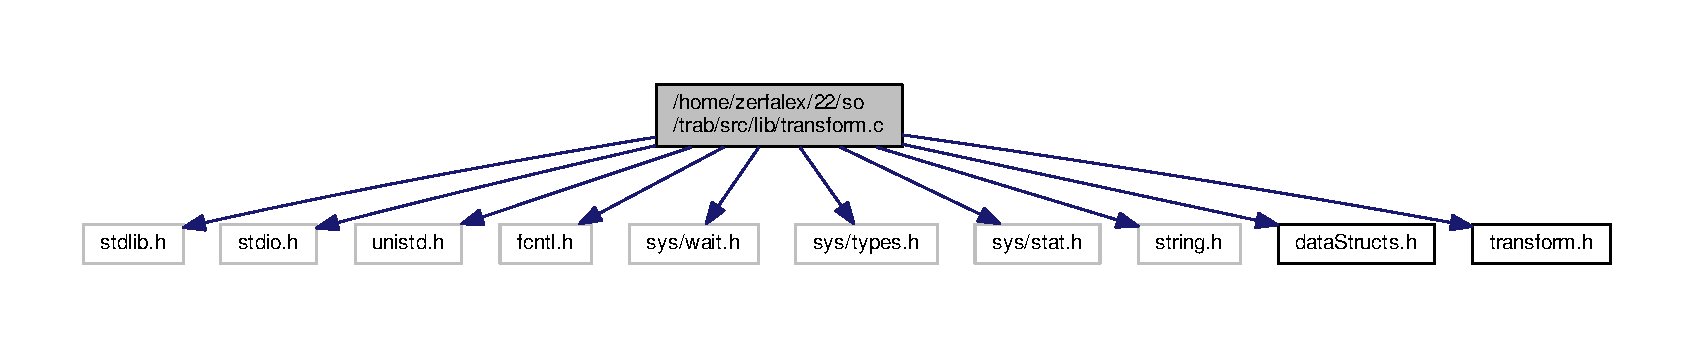
\includegraphics[width=350pt]{transform_8c__incl}
\end{center}
\end{figure}
\subsection*{Functions}
\begin{DoxyCompactItemize}
\item 
void \hyperlink{transform_8c_a41104cfc27eb72adf15afc72b19fc705}{note\+To\+List} (int argc, char $\ast$argv\mbox{[}$\,$\mbox{]}, \hyperlink{data_structs_8h_a02dfe73aee9a117ed44a7abc305f1066}{L\+I\+ST} \hyperlink{structlist}{list})
\item 
void \hyperlink{transform_8c_ac700a91d14c71a5f71c4793ecbfee12d}{list\+To\+Note} (int argc, char $\ast$argv\mbox{[}$\,$\mbox{]}, \hyperlink{data_structs_8h_a02dfe73aee9a117ed44a7abc305f1066}{L\+I\+ST} \hyperlink{structlist}{list})
\end{DoxyCompactItemize}


\subsection{Function Documentation}
\index{transform.\+c@{transform.\+c}!list\+To\+Note@{list\+To\+Note}}
\index{list\+To\+Note@{list\+To\+Note}!transform.\+c@{transform.\+c}}
\subsubsection[{\texorpdfstring{list\+To\+Note(int argc, char $\ast$argv[], L\+I\+S\+T list)}{listToNote(int argc, char *argv[], LIST list)}}]{\setlength{\rightskip}{0pt plus 5cm}void list\+To\+Note (
\begin{DoxyParamCaption}
\item[{int}]{argc, }
\item[{char $\ast$}]{argv\mbox{[}$\,$\mbox{]}, }
\item[{{\bf L\+I\+ST}}]{list}
\end{DoxyParamCaption}
)}\hypertarget{transform_8c_ac700a91d14c71a5f71c4793ecbfee12d}{}\label{transform_8c_ac700a91d14c71a5f71c4793ecbfee12d}


Definition at line 32 of file transform.\+c.

\index{transform.\+c@{transform.\+c}!note\+To\+List@{note\+To\+List}}
\index{note\+To\+List@{note\+To\+List}!transform.\+c@{transform.\+c}}
\subsubsection[{\texorpdfstring{note\+To\+List(int argc, char $\ast$argv[], L\+I\+S\+T list)}{noteToList(int argc, char *argv[], LIST list)}}]{\setlength{\rightskip}{0pt plus 5cm}void note\+To\+List (
\begin{DoxyParamCaption}
\item[{int}]{argc, }
\item[{char $\ast$}]{argv\mbox{[}$\,$\mbox{]}, }
\item[{{\bf L\+I\+ST}}]{list}
\end{DoxyParamCaption}
)}\hypertarget{transform_8c_a41104cfc27eb72adf15afc72b19fc705}{}\label{transform_8c_a41104cfc27eb72adf15afc72b19fc705}


Definition at line 12 of file transform.\+c.


\hypertarget{main_8c}{}\section{/home/zerfalex/22/so/trab/src/main.c File Reference}
\label{main_8c}\index{/home/zerfalex/22/so/trab/src/main.\+c@{/home/zerfalex/22/so/trab/src/main.\+c}}
{\ttfamily \#include $<$stdlib.\+h$>$}\\*
{\ttfamily \#include $<$stdio.\+h$>$}\\*
{\ttfamily \#include $<$unistd.\+h$>$}\\*
{\ttfamily \#include $<$fcntl.\+h$>$}\\*
{\ttfamily \#include $<$sys/wait.\+h$>$}\\*
{\ttfamily \#include $<$sys/types.\+h$>$}\\*
{\ttfamily \#include $<$sys/stat.\+h$>$}\\*
{\ttfamily \#include $<$string.\+h$>$}\\*
{\ttfamily \#include $<$data\+Structs.\+h$>$}\\*
{\ttfamily \#include $<$transform.\+h$>$}\\*
{\ttfamily \#include $<$processor.\+h$>$}\\*
Include dependency graph for main.\+c\+:
\nopagebreak
\begin{figure}[H]
\begin{center}
\leavevmode
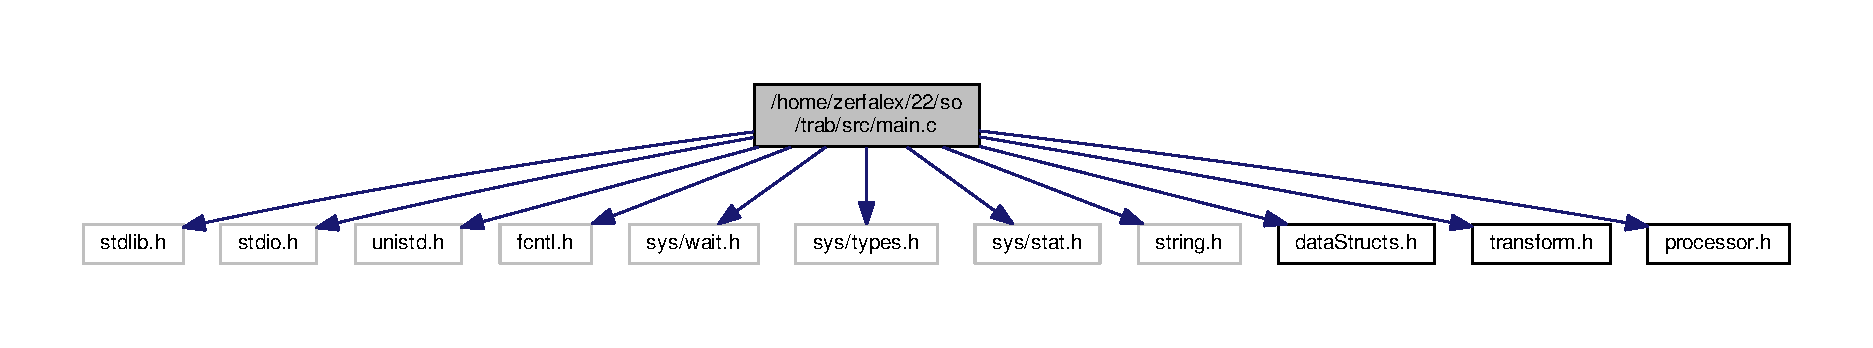
\includegraphics[width=350pt]{main_8c__incl}
\end{center}
\end{figure}
\subsection*{Functions}
\begin{DoxyCompactItemize}
\item 
int \hyperlink{main_8c_a0ddf1224851353fc92bfbff6f499fa97}{main} (int argc, char $\ast$argv\mbox{[}$\,$\mbox{]})
\end{DoxyCompactItemize}


\subsection{Function Documentation}
\index{main.\+c@{main.\+c}!main@{main}}
\index{main@{main}!main.\+c@{main.\+c}}
\subsubsection[{\texorpdfstring{main(int argc, char $\ast$argv[])}{main(int argc, char *argv[])}}]{\setlength{\rightskip}{0pt plus 5cm}int main (
\begin{DoxyParamCaption}
\item[{int}]{argc, }
\item[{char $\ast$}]{argv\mbox{[}$\,$\mbox{]}}
\end{DoxyParamCaption}
)}\hypertarget{main_8c_a0ddf1224851353fc92bfbff6f499fa97}{}\label{main_8c_a0ddf1224851353fc92bfbff6f499fa97}


Definition at line 13 of file main.\+c.


%--- End generated contents ---

% Index
\backmatter
\newpage
\phantomsection
\clearemptydoublepage
\addcontentsline{toc}{chapter}{Index}
\printindex

\end{document}
